
\subsection{Phân tích phương sai hai nhân tố (Two-factor ANOVA)}
\subsubsection{Mục đích}
Trong phần nghiên cứu này, chúng tôi sẽ sử dụng ANOVA 2 yếu tố không lặp để phân tích xem liệu \textbf{Phí giao hàng (delivery\_charges)} và \textbf{Mã giảm giá  (coupon\_discount)} có ảnh hưởng đến \textbf{Chi phí tổng thể (order\_total)} hay không?

Giả thiết thống kê được thực hiện với mức ý nghĩa $\alpha = 0.05$.


\begin{itemize}
    
    \item Kiểm định yếu tố A (delivery\_charges)
    \begin{itemize}
        \item Đánh giá xem biến nhân tố A có ảnh hưởng đến biến phụ thuộc hay không?
        
        \[
            H_{0A}: \tau_{1} = \tau_{2} = \tau_{3} = \dots = \tau_{a} = 0
            \]
            \[
            H_{1A}: \tau_{i} \neq  0 \text{ với ít nhất một i }
            \]
    \end{itemize}
    
    \item Kiểm định yếu tố B (coupon\_discount)
    \begin{itemize}
        \item Đánh giá xem biến nhân tố B có ảnh hưởng đến biến phụ thuộc hay không?
        
        \[
            H_{0B}: \beta_{1} = \beta_{2} = \beta_{3} = \dots = \beta_{b} = 0
            \]
            \[
            H_{1B}: \beta_{j} \neq  0 \text{ với ít nhất một j }
            \]
    \end{itemize}
    \item Đối với tương tác giữa A và B  
    \begin{itemize}
        \item Đánh giá xem các biến nhân tố A và B có ảnh hưởng đến biến phụ thuộc hay không?
        
        \[
            H_{0AB}: \tau\beta_{11} = \tau\beta_{12}  = \dots = \tau\beta_{AB} = 0 
            \]
            \[
            H_{1AB}: \tau\beta_{ij} \neq  0 \text{ với ít nhất một cặp (i,j) }
            \]
    \end{itemize}
\end{itemize}
\subsubsection{Kiểm tra điều kiện cho dữ liệu}
Trước khi tiến hành phân tích ANOVA 2 chiều, chúng tôi cần kiểm tra các điều kiện cần thiết cho dữ liệu thì \textbf{Biến phụ thuộc:} \textbf{order\_total} là một biến không có phân phối chuẩn, tồn tại nhiều khiếm khuyết dữ liệu và có các điểm dị biệt.

$ \Rightarrow $ Như vậy các điều kiện giả thiết về dữ liệu không được thỏa mãn, do đó kết quả phân tích ANOVA có thể không chính xác và chỉ mang tính chất tham khảo.
\subsubsection{Tiến hành phân tích}
Chúng tôi tiến hành phân tích ANOVA 2 chiều trong phần phần mềm r. 

         Kết quả nhận được: 
        
        \begin{figure}[!htbp]
            \centering
            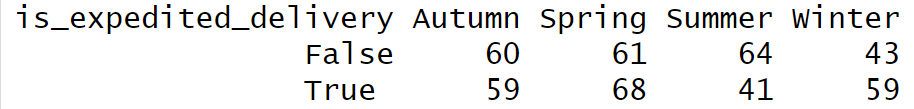
\includegraphics[width=1\linewidth]{graphics/5.4.3.png}
            \caption{Phân tích anova 2 yếu tố}
        \end{figure}
        
        
        Kết quả và nhận xét: 
        Kết quả phân tích ANOVA hai yếu tố được trình bày trong hình 5.4. Kết quả cho thấy rằng cả ba yếu tố \textbf{coupon\_discount}, \textbf{delivery\_charges}, và sự tương tác giữa chúng đều có ảnh hưởng đáng kể đến \textbf{order\_total} với mức ý nghĩa $\alpha = 0.05$. Dưới đây là các nhận xét chi tiết:
        
            \begin{itemize}
    \item \textbf{coupon\_discount}:
    \begin{itemize}
        \item Với \textbf{Df = 4}, có 4 mức độ khác nhau trong yếu tố \textbf{coupon\_discount}.
        \item Giá trị \textbf{F = 973.68} và \textbf{Pr(>F) < 2e-07***} cho thấy rằng sự khác biệt giữa các mức độ của \textbf{coupon\_discount} có ảnh hưởng đáng kể đến \textbf{order\_total}. Do đó, ta bác bỏ giả thuyết không \(H_0\) cho yếu tố này.
    \end{itemize}

    \item \textbf{delivery\_charges}:
    \begin{itemize}
        \item Với \textbf{Df = 467}, có 467 mức độ khác nhau trong yếu tố \textbf{delivery\_charges}.
        \item Giá trị \textbf{F = 945.37} và \textbf{Pr(>F) < 1.09e-07***} cho thấy rằng sự khác biệt giữa các mức độ của \textbf{delivery\_charges} có ảnh hưởng đáng kể đến \textbf{order\_total}. Do đó, ta bác bỏ giả thuyết không \(H_0\) cho yếu tố này.
    \end{itemize}

    \item \textbf{Tương tác giữa coupon\_discount và delivery\_charges}:
    \begin{itemize}
        \item Với \textbf{Df = 23}, có 23 mức độ tương tác giữa hai yếu tố \textbf{coupon\_discount} và \textbf{delivery\_charges}.
        \item Giá trị \textbf{F = 37.84} và \textbf{Pr(>F) = 0.000372***} cho thấy rằng có sự tương tác có ý nghĩa thống kê giữa hai yếu tố này và ảnh hưởng đến \textbf{order\_total}. Do đó, ta bác bỏ giả thuyết không \(H_0\) cho sự tương tác này.
    \end{itemize}

    \item \textbf{Residuals}:
    \begin{itemize}
        \item Số dư tự do còn lại là \textbf{Df = 5}.
        \item Tổng bình phương của sai số là \textbf{Sum Sq = 4.203e+08}.
    \end{itemize}
    \end{itemize}

 Từ những kết quả trên, chúng tôi kết luận rằng cả yếu tố \textbf{coupon\_discount}, \textbf{delivery\_charges}, và sự tương tác giữa chúng đều có ảnh hưởng quan trọng và có ý nghĩa thống kê đối với \textbf{order\_total}. Điều này cho thấy rằng các yếu tố này cần được cân nhắc kỹ lưỡng khi định giá sản phẩm.
               
        
\subsubsection{Kết luận}
Phân tích ANOVA 2 chiều cho thấy \textbf{coupon\_discount}, \textbf{delivery\_charges}, và sự tương tác giữa chúng đều có ảnh hưởng đáng kể đến \textbf{order\_total}. Mặc dù có một số hạn chế về phân phối chuẩn và phương sai không đồng nhất, kết quả này vẫn cung cấp cơ sở tin cậy để đánh giá và điều chỉnh chiến lược giá sản phẩm.